% !TeX encoding = UTF-8
% !TeX spellcheck = en_US
% !TeX root = ../../Thesis.tex

\chapter{Vacuum test chamber}
\label{chap:Vacuum chamber}

Vacuum chamber -> Frank \\
Kurz: Wie sieht die Kammer aus, ev. Wie ist die CRT drinnen gemountet \\
CRT Mount ??


2020-08-30 leak rate
2020-09-27 set voltages
2020-09-30 first successful external run
2020-10-07 spot vs pressure
2020-10-22 current measurement aluminum foil
2020-11-05 forgot to turn off filament heating
2020-11-14 assemble chamber with copper rings


\section{First iteration}
\label{sec:vacuum chamber first iteration}

A vacuum test chamber (\cref{fig:3D rendering of test chamber}) was build to run opened CRTs. In order to be able to fit the CRT screen, CF160 flanges were chosen. The center piece consists of a 6-way cross with view ports at the front and bottom . A valve was installed at the back in order to flood the chamber with nitrogen\todo{pure nitrogen name?} when installing a new CRT. On the right side, a HiCube 300 Eco turbo pump was installed and on the left side a wobble stick attached with a wire. A nipple fitting \todo{length} was installed at the top with a 5 port cluster flange, each being of type CF63. In the middle port a VSH\todo{find exact model \url{https://www.manualslib.com/products/Thyracont-Vsh87d-10434070.html}} vacuum transducer was installed to measure the pressure. This needs a \SI{24}{\volt} dc power supply. On the left, a 19 pin connector \todo{how many pins and model name?} was installed to supply the necessary voltages to the CRT. A flange with four BNC feedthroughs was installed at the front. One of them was connected to the wire installed on the wobble stick while another one was connected to some aluminum foil on the CRT screen (\cref{fig:Wire on wobble stick and aluminum foil}). The other two ports were capped off by blank flanges.

\begin{figure}[ht]
	\centering
	
	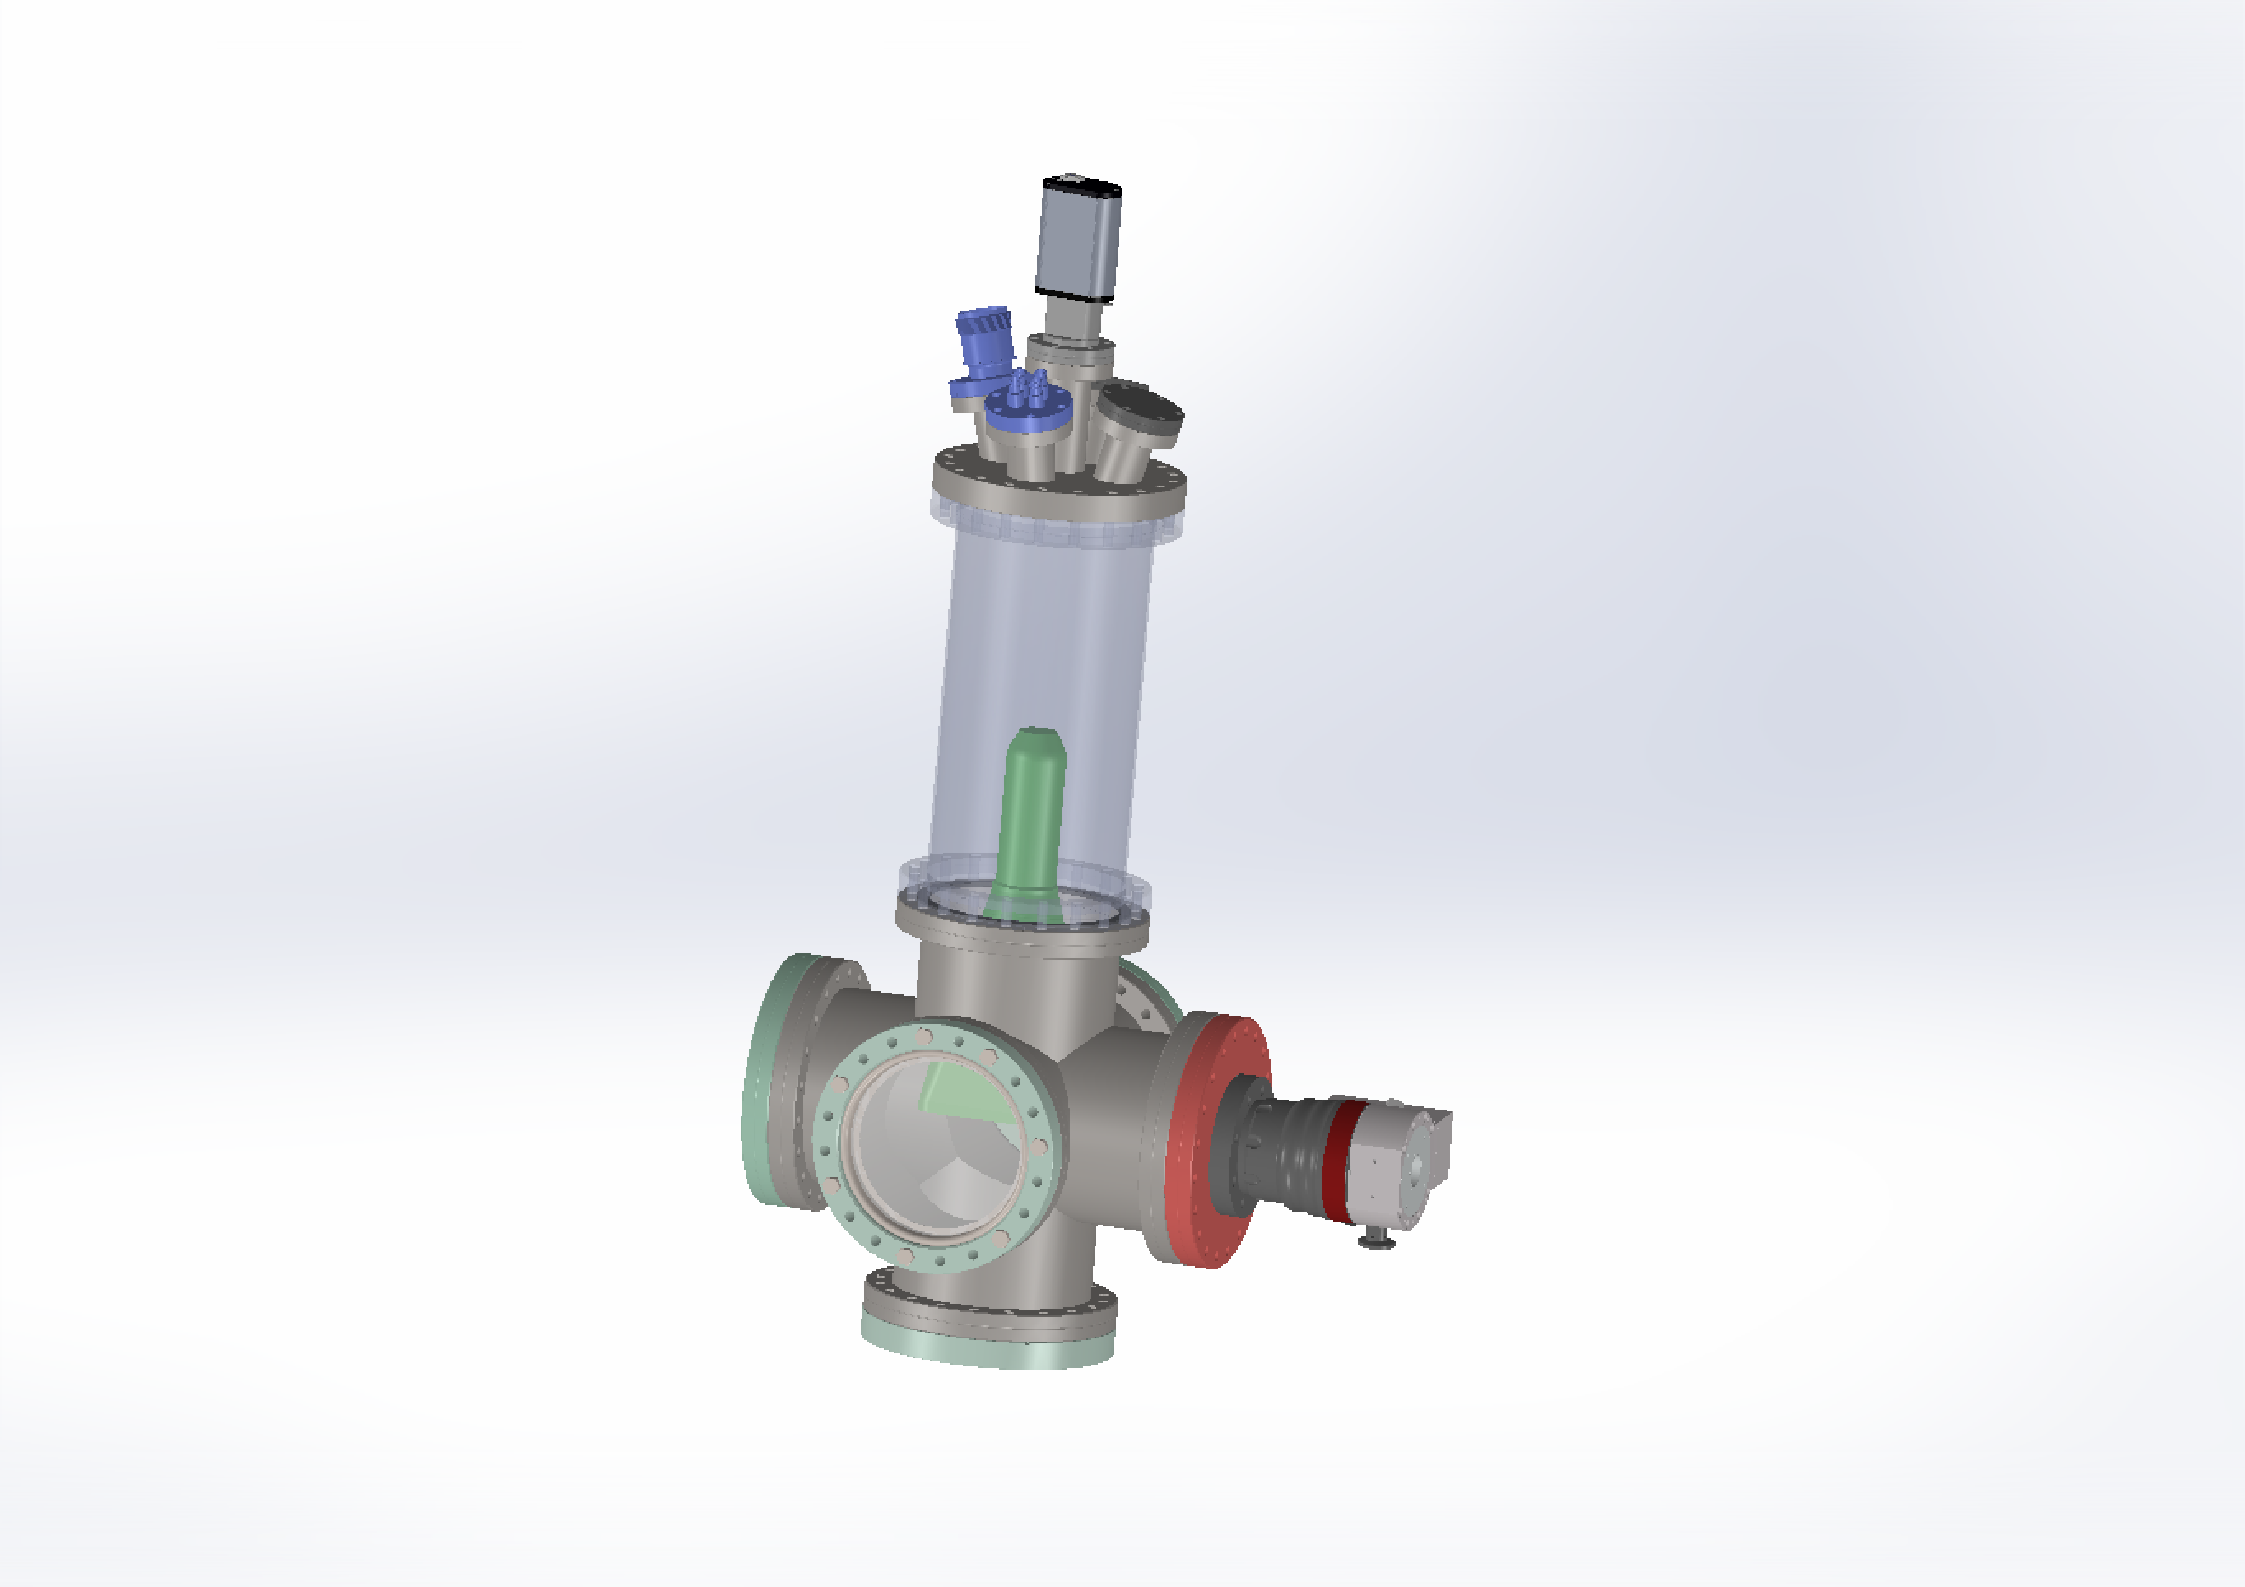
\includegraphics[width=0.9\textwidth]{./Chapters/vacuum-chamber/test_chamber} % taken from OneNote QuaK/Vacuum Setup/Test vacuum chamber
	
	\caption{3D rendering of test chamber.}
	\label{fig:3D rendering of test chamber}
\end{figure}


\begin{figure}[ht]
	\centering
	
	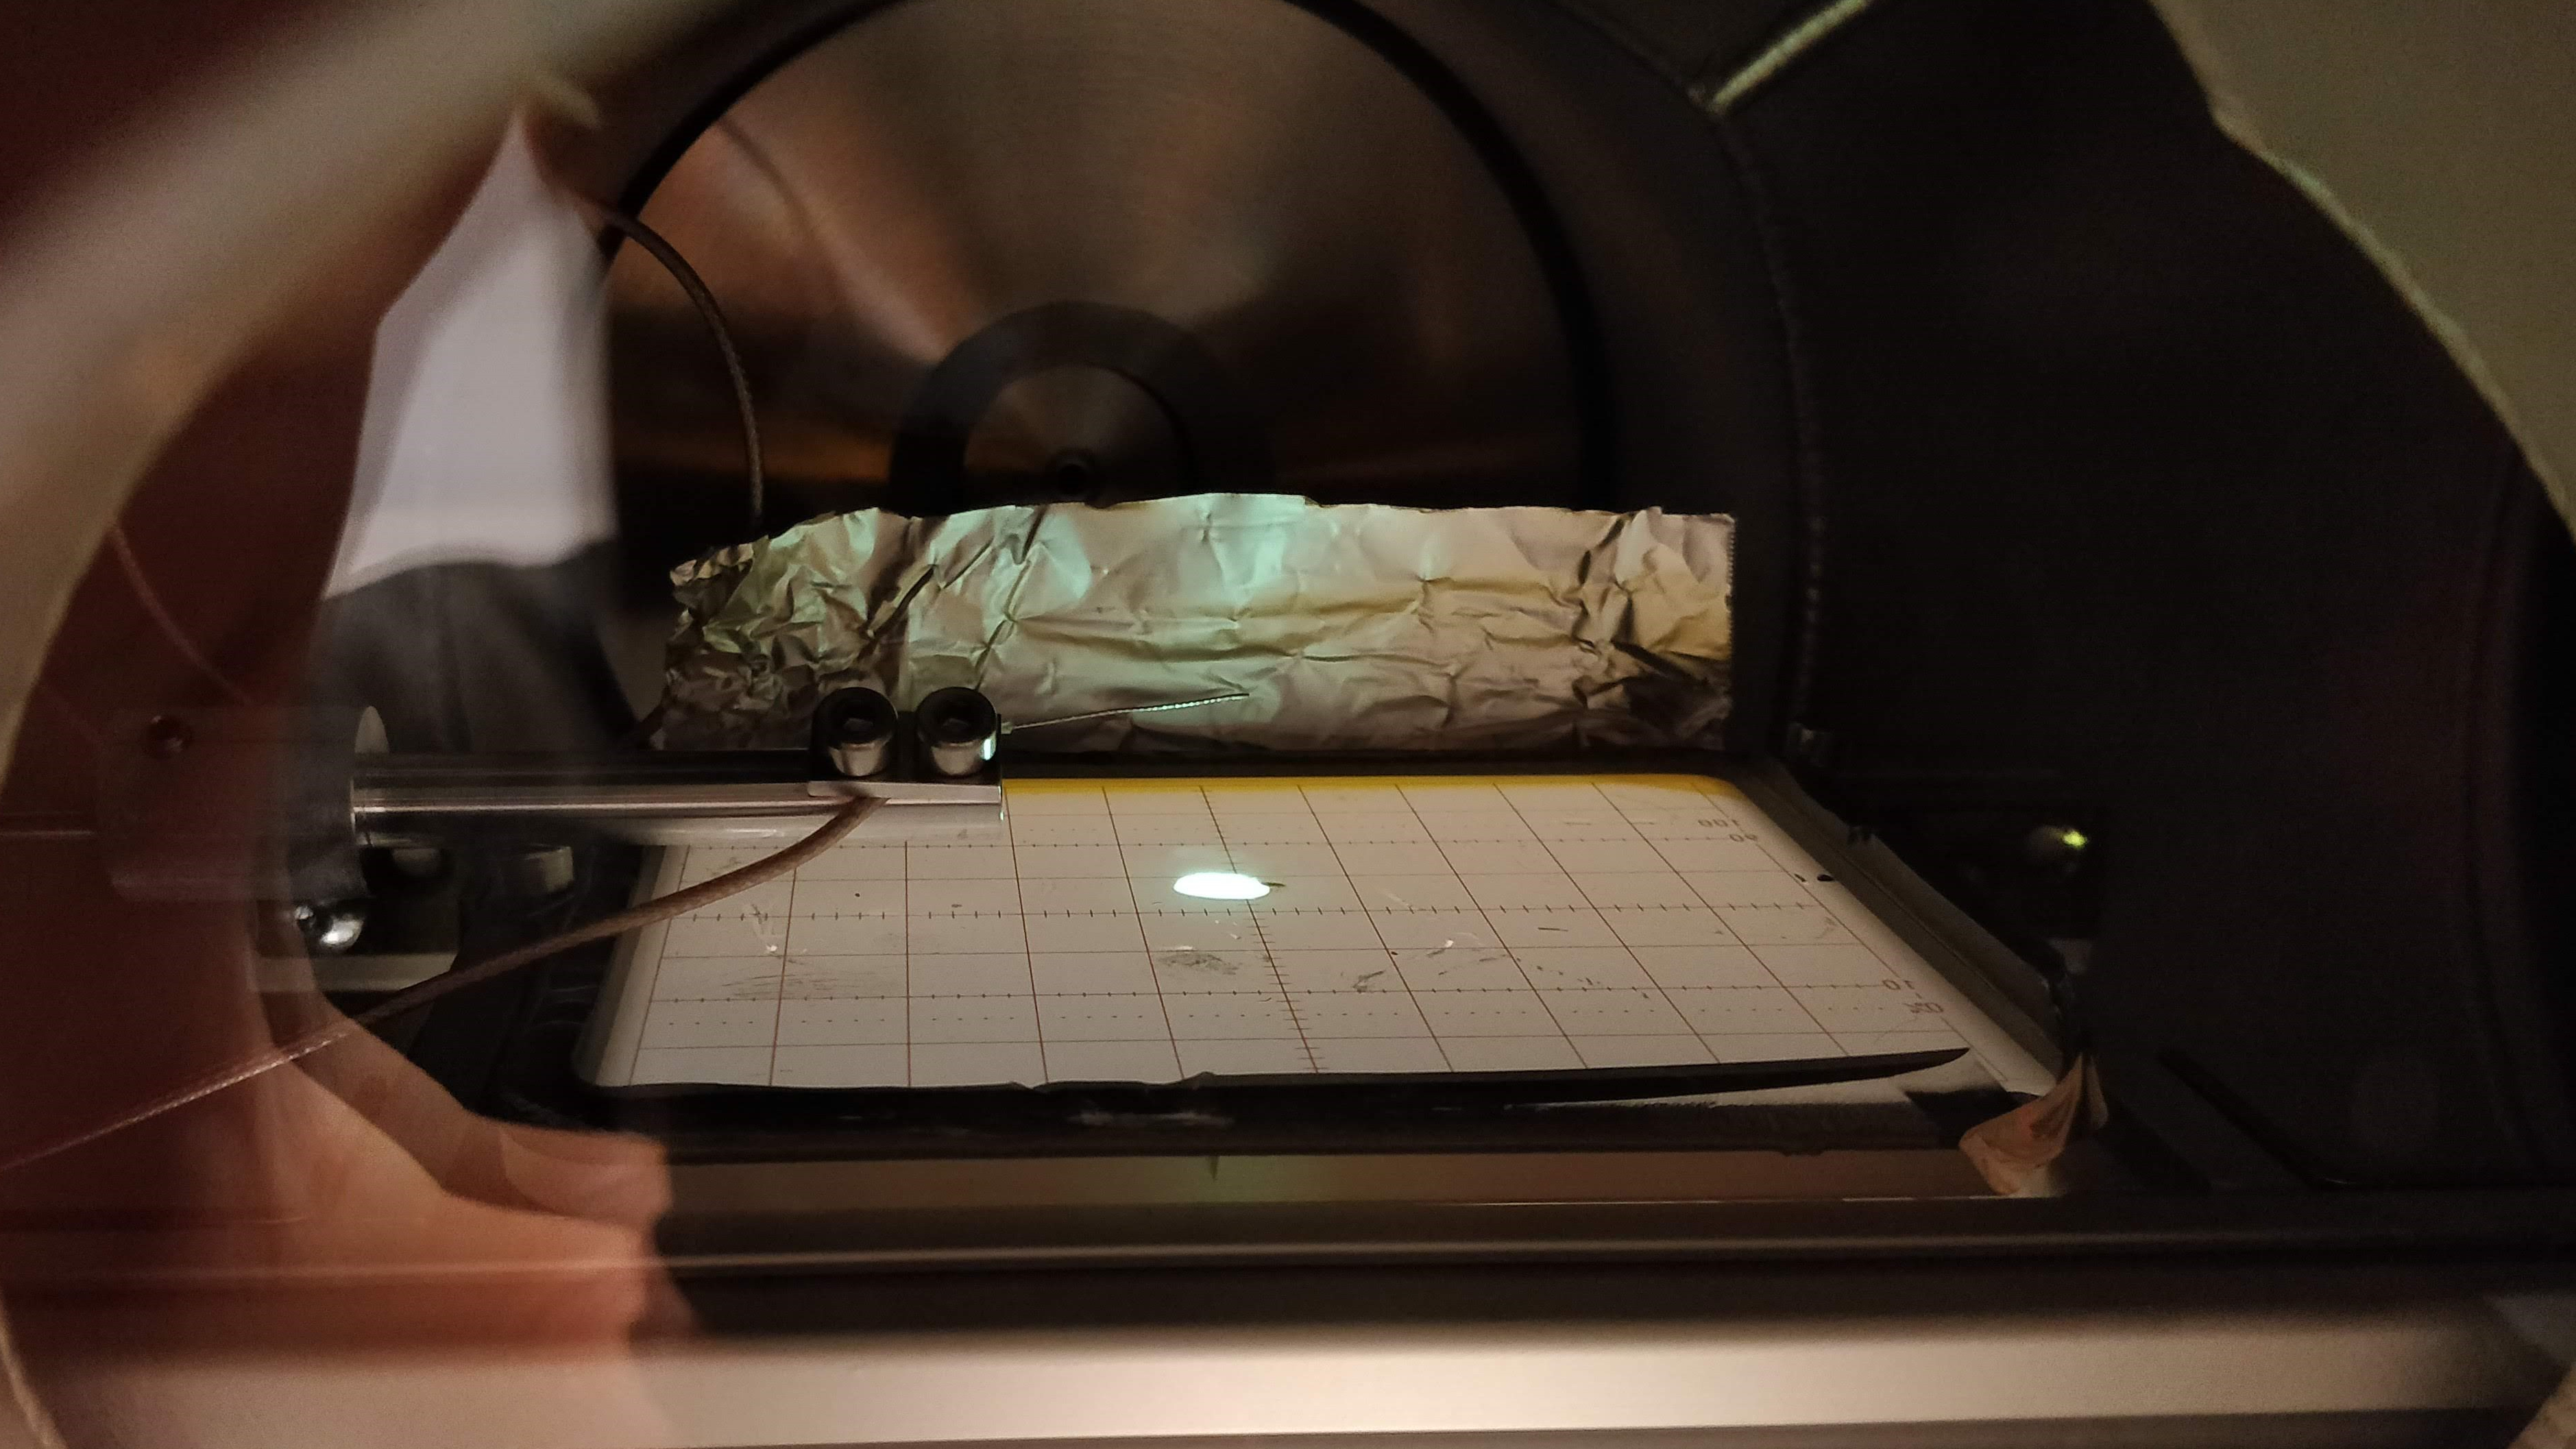
\includegraphics[width=0.9\textwidth]{./Chapters/vacuum-chamber/center_image}
	
	\caption{Wire on wobble stick and aluminum foil.}
	\label{fig:Wire on wobble stick and aluminum foil}
\end{figure}

Before inserting a CRT, a leak test was performed. First, the chamber was set to a pressure of \SI{e-5}{\milli\bar} after which the pump was turned off. The pressure was measured once a minute for a duration \SI{3}{\hour}. The plot is shown in \cref{fig:Leak rate of test chamber after turning off pump}.

\begin{figure}[ht]
	\centering
		
	\begin{tikzpicture}
		% !TeX encoding = UTF-8
% !TeX spellcheck = en_US
% !TeX root = ../../Thesis.tex

\begin{axis}[
	%name=zeemanShift,
	%grid=major,
	ymode = log,
	xlabel = time/\si{\minute},
	ylabel = pressure/\si{\milli\bar},
	%scaled ticks=false,
	%		every x tick scale label/.style={at={(xticklabel* cs:1.03,-0.3em)}, /pgfplots/near ticklabel align=outside, anchor=near xticklabel opposite, inner sep=0pt},
	%		xticklabel style={/pgf/number format/sci}, sci generic={mantissa sep=\cdot,exponent={10^{#1}}}},
	%yticklabel style={/pgf/number format/sci},
	xmin = 0,
	ymin = 1e-5,
	%extra tick style={grid=none}, 
	%width=0.7\textwidth,
	%legend style={at={(1.02, 0.5)}, anchor = west},
	%every axis plot/.append style={thick}
	]
	\addplot[mark=none, black] table [x=t, y=p, col sep=comma]{./Chapters/vacuum-chamber/leak_rate.csv};
\end{axis}
	\end{tikzpicture}
	
	\caption{Leak rate of test chamber after turning off pump.}
	\label{fig:Leak rate of test chamber after turning off pump}
\end{figure}


